\documentclass[a4paper,leqno]{article}
\usepackage[utf8]{inputenc}
\usepackage{lmodern}
\usepackage{microtype}
\usepackage[inline]{enumitem}

\usepackage{siunitx}
\usepackage{multirow}
\usepackage{subcaption}

\usepackage[english]{babel}
\usepackage[autostyle, english=british]{csquotes}
\MakeOuterQuote{"}

\usepackage{commath}
\usepackage{amsmath}
\usepackage{amsthm}
\usepackage{amssymb}
\usepackage{mathtools}

\usepackage{pifont}
\reversemarginpar
\newcommand{\marginsymbol}{\marginpar{\hfill(\ding{43})}}

\usepackage[dvipsnames]{xcolor}
\usepackage{pgfplots}
\pgfplotsset{compat=1.11}
\usepgfplotslibrary{fillbetween}
\usetikzlibrary{patterns}
\usetikzlibrary{arrows}
\usepgfplotslibrary{statistics}

\newcommand*{\SectorRadius}{1.5ex}
\newcommand*{\SectorHalfAngle}{45}
\newcommand*{\SectorLineWidth}{.4pt}

\newcommand*{\sector}{%
  \begin{pgfpicture}
    \pgfpathmoveto{\pgforigin}%
    \pgfpathlineto{\pgfpointpolar{90-(\SectorHalfAngle)}{\SectorRadius}}%
    \pgfarc{90-(\SectorHalfAngle)}{90+\SectorHalfAngle}{\SectorRadius}%
    \pgfpathclose
    \pgfsetlinewidth{\SectorLineWidth}%
    \pgfusepath{stroke}%
  \end{pgfpicture}%
}

\PassOptionsToPackage{hyphens}{url}
\usepackage{hyperref}

\usepackage[margin=1in]{geometry}
\usepackage{changepage}
\usepackage{titlesec}
\titleformat{\section}{\normalfont\Large\bfseries\centering}{Section~\thesection:}{1em}{}

\def\signed #1{{\leavevmode\unskip\nobreak\hfil\penalty50\hskip2em
  \hbox{}\nobreak\hfil(#1)%
  \parfillskip=0pt \finalhyphendemerits=0 \endgraf}}
\newsavebox\mybox
\newenvironment{aquote}[1]
  {\savebox\mybox{#1}\begin{quote}}
  {\signed{\usebox\mybox}\end{quote}}

% Augmented matrices.
\makeatletter
\renewcommand*\env@matrix[1][*\c@MaxMatrixCols c]{%
  \hskip -\arraycolsep
  \let\@ifnextchar\new@ifnextchar
  \array{#1}}
\makeatother

% russian integral
\usepackage{scalerel}
\DeclareMathOperator*{\rint}{\scalerel*{\rotatebox{17}{$\!\int\!$}}{\int}}

%--------grstep
% For denoting a Gauss' reduction step.
% Use as: \grstep{\rho_1+\rho_3} or \grstep[2\rho_5 \\ 3\rho_6]{\rho_1+\rho_3}
\newcommand{\grstep}[2][\relax]{%
   \ensuremath{\mathrel{
       {\mathop{\longrightarrow}\limits^{#2\mathstrut}_{
                                     \begin{subarray}{l} #1 \end{subarray}}}}}}
\newcommand{\swap}{\leftrightarrow}


\swapnumbers
\numberwithin{equation}{section}
\newtheorem{thm}[equation]{Theorem}
\newtheorem{lem}[equation]{Lemma}
\newtheorem{cor}[equation]{Corollary}
\newtheorem{prp}[equation]{Proposition}
\theoremstyle{definition}
\newtheorem{defn}[equation]{Definition}
\newtheorem{notation}[equation]{Notation}
\newtheorem{ex}[equation]{Example}
\newtheorem{exercise}[equation]{Exercise}
\newtheorem{alg}[equation]{Algorithm}
\theoremstyle{remark}
\newtheorem{rem}[equation]{Remark}

\newcommand{\df}{\textbf}

\newcommand{\union}{\cup}
\newcommand{\inter}{\cap}

\title{Level Three Statistics}
\author{Alex Elzenaar}
\date{\today}

\begin{document}
\maketitle
\tableofcontents
\section*{Preface}
These notes are intended to be a basic introduction to statistics for L3 and Scholarship students. Section 1, on probability measures, follows
Rice\footnote{The references here are to the bibliography at the end of these notes.}; section 2 on distributions follows Wackerly, Mendenhall,
and Sheaffer; and section 3 on inference follows Efron and Tibsirai.

\titleformat{\section}{\clearpage\titlerule[0.8pt]\vspace{0.5ex}\normalfont\Large\bfseries\centering}{Section~\thesection:}{1em}{}[{\titlerule[0.8pt]}]
\let\oldsection\section
\renewcommand\section{\clearpage\oldsection}
\section{Probability}
\subsection{Foundations}
Probability theory is the study of events which occur randomly. The situations within which such events occur are called \df{experiments}; the set
of all possible outcomes of an experiment is called the \df{sample space} of the experiment. We will generally use $ \Omega $ to denote sample
spaces.

\begin{ex}
  Flipping a coin three times is an experiment with sample space
  \begin{displaymath}
    \Omega = \{HHH, HHT, HTH, THH, HTT, THT, TTH, TTT\}.
  \end{displaymath}
\end{ex}

Particular subsets of sample spaces are called \df{events}. An event is said to \df{occur} if
one the outcomes contained within it occurs. If $ A $ is a subset of $ \Omega $ we write $ A \subseteq \Omega $.

\begin{ex}
  In the coin-flipping experiment, the event `heads occurs twice' is the subset
  \begin{displaymath}
    A = \{HHT, HTH, THH\}.
  \end{displaymath}
  The event `at least one tail is flipped' is the subset
  \begin{displaymath}
    B = \{HHT, HTH, THH, HTT, THT, TTH, TTT\}.
  \end{displaymath}
\end{ex}

\begin{defn}[Set-theoretic operations]
  If $ A $ and $ B $ are events in the sample space $ \Omega $, then:-
  \begin{enumerate}
    \item The \df{union} of $ A $ and $ B $, denoted $ A \union B $, is the event that either $ A $, or $ B $, or both occurs. In the
          example above, $ A \union B = \{HHT, HTH, THH, HTT, THT, TTH, TTT\} $ (all outcomes contained within at least one of $ A $ and $ B $).
    \item The \df{intersection} of $ A $ and $ B $, denoted $ A \inter B $, is the event that both $ A $ and $ B $ occur. In the example
          above, $ A \inter B = \{HHT, HTH, THH\} $ (all outcomes contained within both $ A $ and $ B $).
    \item The \df{complement} of $ A $, denoted $ A^\complement $, is the event that $ A $ does not occur. In the example above,
          $ A^\complement = \{HHH, HTT, THT, TTH, TTT\} $ (all outcomes contained in $ \Omega $ but not $ A $).
    \item The \df{empty set} is the event with no outcomes: $ \emptyset = \{\} $. If $ A $ and $ B $ have no common outcomes
          then $ A \inter B = \emptyset $, and $ A $ and $ B $ are called \df{disjoint}.
  \end{enumerate}
\end{defn}

\begin{exercise}
  Draw Venn diagrams to illustrate the following laws:
  \begin{enumerate}
    \item $ A \inter B = B \inter A $ and $ A \union B = B \union A $
    \item $ (A \inter B) \inter C = A \inter (B \inter C) $ and $ (A \union B) \union C = A \union (B \union C) $
    \item $ (A \inter B) \union C = (A \union C) \inter (B \union C) $ and $ (A \union B) \inter C = (A \inter C) \union (B \inter C) $
  \end{enumerate}
\end{exercise}

\begin{defn}\label{df:probmeasure}
  A \df{probability measure} on a sample space $ \Omega $ is a function $ P $ from the subsets of $ \Omega $ to the real numbers
  that satisfies the following axioms:
  \begin{enumerate}
    \item $ P(\Omega) = 1 $
    \item If $ A \subseteq \Omega $ then $ P(A) \geq 0 $
    \item If $ A $ and $ B $ are disjoint then $ P(A \union B) = P(A) + P(B) $.
  \end{enumerate}
\end{defn}

\begin{prp}[Probability calculus]\label{prp:probcalc}\leavevmode
  \begin{enumerate}
    \item $ P(A^\complement) = 1 - P(A) $
    \item $ P(\emptyset) = 0 $
    \item If $ A \subseteq B $ then $ P(A) \leq P(B) $
    \item $ P(A \union B) = P(A) + P(B) - P(A \inter B) $
  \end{enumerate}
\end{prp}
\begin{proof}\leavevmode
  \begin{enumerate}
    \item $ A $ and $ A^{\complement} $ are disjoint, and $ A \union A^{\complement} = \Omega $,
          so $ 1 = P(\Omega) = P(A \union A^{\complement}) = P(A) + P(A^{\complement}) $ and $ P(A^\complement) = 1 - P(A) $.
    \item $ \emptyset^\complement = \Omega $ so $ P(\emptyset) = 1 - P(\emptyset^\complement) = 1 - P(\Omega) = 1 - 1 = 0 $.
    \item If $ A \subseteq B $ then $ B = A \union (B \inter A^\complement) $ where the two unioned sets are disjoint, and
          thus $ P(B) = P(A) + P(B \inter A^\complement) \geq P(A) $ (since $ P(B \inter A^\complement) \geq 0 $).
    \item The idea is that if $ P(A) $ and $ P(B) $ are added together then $ P(A\inter B) $ is double-counted. (Draw a Venn diagram).
          Hence we will write $ A \union B = (A \inter B^\complement) \union (A \inter B) \union (A^\complement \inter B) $ (the unions
          here are disjoint) and so $ P(A \union B) = P(A \inter B^\complement) + P(A \inter B) + P(A^\complement \inter B) $. On the
          other hand, $ P(A) = P(A \inter B^\complement) + P(A \inter B) $, and $ P(B) = P(A \inter B) + P(A^\complement \inter B) $.
          Thus $ P(A) + P(B) - P(A \inter B) = P(A \inter B^\complement) + P(A \inter B) + P(A^\complement \inter B) = P(A \union B) $.
  \end{enumerate}
\end{proof}

\begin{ex}
  If a coin is thrown twice then $ \Omega = \{HH,HT,TH,TT\} $. Assume that each outcome in $ \Omega $ is equally likely and
  has probability $ 1/4 $. Let $ A $ denote the event of heads on the first toss, and $ B $ denote the event of heads on the
  second toss. Then $ 3/4 = P(\{HH,HT,TH\}) = P(A \union B) = P(A) + P(B) - P(A \inter B) = P(\{HH,HT\}) + P(\{HH,TH\}) - P(\{HH\}) = 3/4 $.
\end{ex}

\begin{rem}
  A probability measure function is a kind of area: set up a correspondence between the full sample
  space $ \Omega $ and a unit square $ \square $ of area 1. Then events $ A \subseteq \Omega $ correspond exactly
  to subsets of the square $ F \subseteq \square $ such that $ P(A) $ equals the area of $ F $.

  Compare the properties listed in definition \ref{df:probmeasure} and proposition \ref{prp:probcalc} with
  the axioms for a Jordan area function.\footnote{See, for example, chapter 8 of Lynn Loomis and Schlomo
  Sternberg, \emph{Advanced calculus} (revised edn.). World Scientific (2014).s}
\end{rem}

\subsection{Counting}
For finite sample spaces, the following is easy:
\begin{lem}
  If $ \Omega $ is finite with $ N $ elements, and if every outcome of $ \Omega $ is equally likely, each outcome
  has probability $ 1/N $; if an event $ A \subseteq \Omega $ can occur in any one of $ n $ mutually exclusive ways
  then $ P(A) = n/N $.
\end{lem}

\begin{exercise}[Simpson's paradox]\leavevmode
  \begin{enumerate}
    \item A black urn contains 5 red and 6 green balls, and a white urn contains 3 red and 4 green balls. You are allowed
          to choose an urn and then choose a ball at random from that urn. If you choose a red ball, you win a prize. Which urn
          should you choose to draw from? (Hint: black)
    \item Consider another game; this time the black urn has 6 red and 3 green, and the white urn has 9 red and 5 green. Which
          urn should you choose? (Hint: black)
    \item In the final game, the contents of the second black urn are added to the first black urn, and the contents of the second
          white urn are added to the first white urn. By considering the results to (1) and (2) above, guess which urn should you now pick. Check your answer.
  \end{enumerate}
\end{exercise}

\begin{prp}[Multiplication principle]\label{prp:mult}
  If one experiment has $ m $ outcomes, and a second has $ n $ outcomes, then there are $ mn $ possible outcomes for the two experiments.
\end{prp}
\begin{proof}
  Denote the outcomes of the first experiment by $ a_1,...,a_m $ and the outcomes of the second by $ b_1,...,b_n $. Then the outcomes
  of the combination fill exactly an $ m \times n $ array in which the pair $ a_i b_j $ is in the $ i$th row and $ j$th column.
\end{proof}

\begin{exercise}
  An 8-bit binary word is a sequence of eight binary digits. How many different 8-bit words are there?
\end{exercise}

\begin{defn}
  A \df{permutation} is an ordered arrangement of objects. Suppose from the set $ X = \{x_1,...,x_n\} $ we choose $ r $ elements
  and list them \emph{in order}. If no duplication is allowed, we say we are \df{sampling without replacement}. If we may choose elements
  more than once, we say we are \df{sampling with replacement}.
\end{defn}

The proof of the following is an exercise.

\begin{lem}
  The number of orderings of a set with $ n $ elements is $ n(n-1)\cdots2\cdot1 $. This number is denoted $ n! $ and
  is called $ n $--\df{factorial}.
\end{lem}

\begin{thm}[Elementary counting theorem, part I]
  For a set of size $ n $ and a sample of size $ r $:
  \begin{enumerate}
    \item there are $ n^r $ different ordered samples with replacement;
    \item there are $ n(n-1)\cdots(n - r + 1) = \frac{n!}{(n - r)!} $ different ordered samples without replacement.
  \end{enumerate}
\end{thm}
\begin{proof}
  We will use the multiplication principle, proposition \ref{prp:mult}. If we allow replacement, the first item in the sample can be chosen $ n $
  different ways; the second $ n $ different ways; and so forth for all $ r $ elements. Thus there are $ \underbrace{n \cdots n}_{r\text{ times}} = n^r $
  samples with replacement.

  Without replacement, we may choose the first element $ n $ ways; the second $ n - 1 $ ways; and so forth, until we are left with $ n - r + 1 $ choices
  for the $ r$th element.
\end{proof}

\begin{exercise}\leavevmode
  \begin{enumerate}
    \item How many ways can five children be lined up?
    \item How many ways is it to choose five children from a group of ten, and line them up?
    \item How many distinct license plates, made up of three letters followed by three digits, are possible?
    \item If all sequences of six characters are equally likely, what is the probability that a license
          plate for a car contains no duplicate letters or numbers?
    \item (Birthday problem) Suppose that a room contains $ n $ people. What is the probability that at least two of them share a birth date?
    \item How many people must you ask to have a 50:50 chance of finding someone who shares your birthday?
  \end{enumerate}
\end{exercise}

\begin{thm}[Elementary counting theorem, part II]
  The number of unordered samples of $ r $ objects selected from $ n $ objects without replacement is
  \begin{displaymath}
    \binom{n}{r} := \frac{n!}{(n - r)!r!}.
  \end{displaymath}
  Alternatively, this is the number of subsets of size $ r $ that can be found in a set of size $ n $.

  The number $ \binom{n}{r} $ is called a \df{binomial coefficient}.
\end{thm}
\begin{proof}
  The number of unordered samples of $ r $ objects selected from $ n $ objects without replacement is just
  the number of ordered such samples, divided by the number of times each unordered sample occurs (this is just
  the number of orderings of a sample of size $ r $). Thus we obtain
  \begin{displaymath}
    \frac{\frac{n!}{(n - r)!}}{r!} = \frac{n!}{(n - r)!r!}.
  \end{displaymath}
\end{proof}

\begin{cor}[Binomial theorem]
  \begin{displaymath}
    (a + b)^n = \binom{n}{0} a^n b^{0} + \binom{n}{1} a^{n - 1} b^{1} + \cdots + \binom{n}{r} a^{n - r} b^r + \cdots + \binom{n}{n} a^{0} b^n.
  \end{displaymath}
\end{cor}

\begin{cor}
  There are $ 2^n $ subsets of a set with $ n $ elements:
  \begin{displaymath}
    2^n = \binom{n}{0} + \binom{n}{1} + \cdots + \binom{n}{n}
  \end{displaymath}
\end{cor}

\begin{exercise}
  A monkey at a typewriter types each of the 26 letters of the alphabet exactly once in a random order. What is
  the probability that the word `hamlet' occurs somewhere in the string of letters?
\end{exercise}

\begin{exercise}
  When performing quality control, only a fraction of the output of a process is sampled and checked.
  Suppose that $ n $ items are produced, and a sample of size $ r $ is chosen and examined. Suppose that the
  entire production contains $ k $ defective items. What is the probability that the sample contains
  exactly $ m $ defective items?
\end{exercise}

\subsection{Conditional probability}
\begin{defn}
  Let $ A $ and $ B $ be events, and let $ P(B) \neq 0 $. Then the \df{conditional probability} of $ A $ given $ B $ is defined to be
  \begin{displaymath}
    P(A | B) = \frac{P(A \inter B)}{P(B)}.
  \end{displaymath}
\end{defn}
The idea is that if we know that $ B $ has occured, our sample space is now only the outcomes in $ B $ rather than the entirity of $ \Omega $.

\begin{exercise}
  Is it true that if the occurence of $ A $ makes $ B $ more likely to occur, then the occurence of $ B $
  makes $ A $ more likely to occur? In other words, if $ P(B|A) > P(B) $ does it follow that $ P(A | B) > P(A) $?
\end{exercise}

The following is trivial but often useful.
\begin{lem}[Multiplication law]
  $ P(A \inter B) = P(A | B) P(B) $.
\end{lem}

\begin{ex}
  An urn contains three red balls and one blue ball. Two balls are selected without replacement. What is the probability that both are red?

  Let $ A $ denote the event `the first ball drawn is red', and $ B $ denote `the second ball drawn is red'. Then $ P(A) = 3/4 $;
  and $ P(B | A) = 2/3 $ (if one red ball has been drawn, there are two left out of three). So $ P(A \inter B) = (3/4)(2/3) = 1/2 $.
\end{ex}

\begin{exercise}
  If it is cloudy, the probability of rain is 0.3. The probability that it is cloudy is 0.2. What is the probability
  that it is cloudy and raining?
\end{exercise}

If $ A $ is any event, and if we can find $ n $ distinct `pathways' that could get to $ A $ such that at least one pathway occurs, we can
find the probability of $ A $.

\begin{thm}{Law of total probability}
  Let $ B_1, B_2,...,B_n $ be mutually disjoint events such that $ B_1 \union \cdots \union B_n = \Omega $. Suppose that $ P(B_i) > 0 $
  for all $ i $. If $ A $ is any event, we have
  \begin{displaymath}
    P(A) = P(A | B_1) P(B_1) + P(A | B_2) P(B_2) + \cdots + P(A | B_n) P(B_n).
  \end{displaymath}
\end{thm}
\begin{proof}
  \begin{align*}
    P(A) = P(A \inter \Omega) &= P\left(A \inter (B_1 \union B_2 \union \cdots \union B_n)\right)\\
                              &= P\left((A \inter B_1) \union \cdots \union (A \inter B_n)\right)\\
                              &= P(A \inter B_1) + \cdots + {(A \inter B_n)}\\
                              &= P(A | B_1) P(B_1) + \cdots + P(A | B_n) P(B_n).
  \end{align*}
\end{proof}

\begin{ex}\label{ex:totalprob1}
  An urn contains three red balls and one blue ball. Two balls are selected without replacement. What is the probability that
  a red ball is selected in the second draw?

  Let $ A $ be the event ``a red ball is selected in the second draw''; let $ B_1 $ be the event ``a red ball is selected
  in the first draw''; let $ B_2 $ be the event ``a blue ball is selected in the first draw''.

  Then $ P(A|B_1) = 2/3 $ (since if a red ball was drawn there are two reds and one blue left), $ P(A | B_2) = 1/1 $,
  $ P(B_1) = 3/4 $, and $ P(B_2) = 1/4 $; thus the law of total probability tells us that $ P(A) = (2/3)(3/4) + (1/1)(1/4) = 3/4 $.
\end{ex}

\begin{figure}
  \centering
  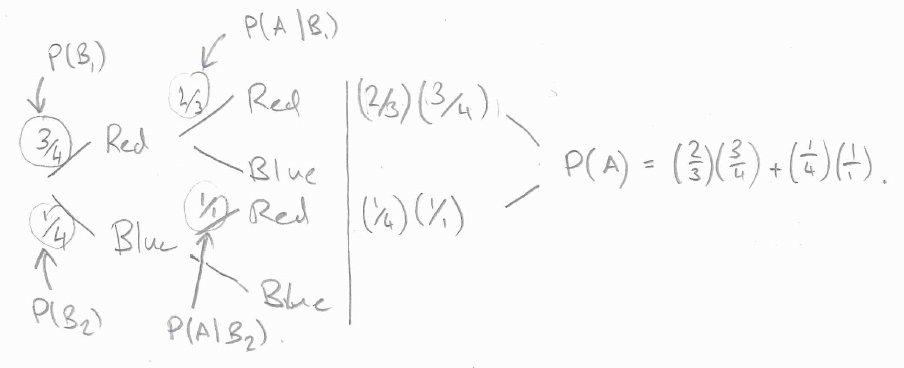
\includegraphics[width=0.6\textwidth]{pt1}
  \caption{Probability tree for example \ref{ex:totalprob1}.\label{fig:pt1}}
\end{figure}

\begin{rem}
  The law of total probability is simply a symbolic version of the method of `probability trees', taught at Level 2. An annotated
  probability tree for the previous example is given in figure \ref{fig:pt1}.
\end{rem}

\begin{exercise}\leavevmode
  \begin{enumerate}
    \item Urn A contains four red, three blue, and two green balls. Urn B has two red, three blue,
          and four green balls. A ball is drawn from urn A and put into urn B, and then a ball is
          drawn from urn B.
      \begin{enumerate}
        \item What is the probability that a red ball is drawn from urn B?
        \item If a red ball is drawn from urn B, what is the probability that
              a red ball was drawn from urn A?
      \end{enumerate}
    \item A couple has two children. What is the probability that both are girls given that
      \begin{enumerate}
        \item the oldest is a girl?
        \item one of them is a girl?
      \end{enumerate}
    \item A fair coin is tossed three times.
      \begin{enumerate}
        \item Given that there was at least one head, what is the probability that at least two heads were thrown?
        \item Given that there was at least one \emph{tail}, what is the probability that at least two heads were thrown? (The second `head' is not a typo.)
      \end{enumerate}
    \item Adam and Brandi are playing the following game. They write each number from 1 to 100 on seperate pieces of paper;
          then they randomly select one piece of paper, and then another. They add the two integers that are written on the
          two pieces of paper. If the sum is even, Adam wins. If the sum is odd, Brandi wins. Is the game fair? Replacing `100'
          with $ n $, for which values of $ n $ is the game fair?
    \item Five cards are dealt from a standard 52-card deck, and the first one is a kind. What is the probability
          of at least one more king?
    \item (Monty Hall problem.) You are shown three doors; behind each door lies either a goat or a unicorn. There are two goats, and one unicorn;
          the object of the game is to end up with the unicorn.

          First, you pick one of the doors, but you are not shown whether a goat or a unicorn is behind it. If only one of the remaining doors hides
          a goat, it is opened. If both remaining doors hide goats, one is picked at random and opened. This leaves two unopened doors: the one
          you picked originally, and the door that you did not pick and which has not been opened to reveal a goat.

          You are given a choice: you may either stick with your original choice, or swap to the door that you did not pick and which remains unopened.
          Does it matter?
    \item Show that if $ P(A | E) \geq P(B | E) $ and $ P(A | E^\complement) \geq P(B | E^\complement) $ then $ P(A) \geq P(B) $.
    \item Show that, if the conditional probabilities exist,
      \begin{displaymath}
        P(A_1 \inter A_2 \inter \cdots \inter A_n) = P(A_1) P(A_2 | A_1) P(A_3 | A_1 \inter A_2) \cdots P(A_n | A_1 \inter \cdots \inter A_{n-1}).
      \end{displaymath}
  \end{enumerate}
\end{exercise}

We have stated laws which allow us to, given conditional probabilities, find probabilities on the entire sample space $ \Omega $. As
is often the case, the inverse problem is more difficult (division is more difficult than multiplication, antidifferentiation is more difficult
than differentiation, ...). One of the most wonderful results of elementary probability, therefore, is the following theorem.

\begin{thm}[Bayes]
  Let $ B_1, B_2,...,B_n $ be mutually disjoint events such that $ B_1 \union \cdots \union B_n = \Omega $. Suppose that $ P(B_i) > 0 $
  for all $ i $. If $ A $ is any event, we have
  \begin{displaymath}
    P(B_j | A) = \frac{P(A | B_j) P(B_j)}{P(A | B_1) P(B_1) + \cdots + P(A | B_n) P(B_n)}
  \end{displaymath}
\end{thm}
\begin{proof}
  Behold:-
  \begin{displaymath}
    P(B_j | A) = \frac{P(A \inter B_j)}{P(A)} = \frac{P(A | B_j) P(B_j)}{P(A | B_1) P(B_1) + \cdots + P(A | B_n) P(B_n)}
  \end{displaymath}
  (where the second equality comes from the multiplication law on the top and the law of total probability below).
\end{proof}

\subsection{Independence}
Two events $ A $ and $ B $ should be independent if the knowledge that $ B $ has occured does not provide any information
as to the occurance of $ A $ (and vice versa); symbolically, if $ P(A | B) = P(A) $ and $ P(B | A) = P(B) $. By the previous
section, the first of these implies that $ P(A) = P(A | B) = P(A \inter B)/P(B) $. We will use this as our definition.

\begin{defn}
  Two events $ A $ and $ B $ are called \df{pairwise independent} if $ P(A \inter B) = P(A) P(B) $.
\end{defn}
\begin{ex}
  A card is randomly selected from a deck. Let $ A $ be the event that the card is an ace, and let $ D $ be the event that the
  card is a diamond. We have $ P(A) = 1/13 $, $ P(D) = 1/4 $, and $ P(A \inter D) = 1/52 $. But $ P(A) P(D) = 1/(13 \cdot 4) = 1/52 = P(A \inter D) $,
  so the two events are independent.
\end{ex}

Warning: if more than two events are considered, it is possible that the entire collection is not independent even though
every pair is pairwise independent.

\begin{ex}
  Let a fair coin be tossed twice, and let the events $ A $, $ B $, $ C $ be `heads on the first toss', `heads on the second toss',
  and `exactly one head is thrown' respectively. Then $ A $ and $ B $ are independent by assumption of fairness; also, $ P(C | A) = 0.5 = P(C) $,
  and $ P(C | B) = 0.5 = P(C) $. Thus all three events are pairwise independent. But $ P(A \inter B \inter C) = 0 \neq P(A)P(B)P(C) $.
\end{ex}

Because of this, we will make a further definition.
\begin{defn}
  A collection of events $ A_1,...,A_n $ are called \df{mutually independent} if $ P(A_1 \inter\cdots \inter A_n) = P(A_1) \cdots P(A_n) $.
\end{defn}

\begin{exercise}\leavevmode
  \begin{enumerate}
    \item Show that if $ A $ and $ B $ are (pairwise) independent, then $ A $ and $ B^\complement $ are pairwise independent,
          and $ A^\complement $ and $ B $ are pairwise independent.
    \item If $ A $ and $ B $ are disjoint, can they be independent? If $ A \subseteq B $, can $ A $ and $ B $ be independent?
    \item If a parent has genotype $ Aa $, they transmit either $ A $ or $ a $ to an offspring (each with a 0.5 chance). The gene
          transmitted to one offspring is independent of the gene transmitted to another. Consider a parent with three children
          and the following events: $ A $, `children 1 and 2 have the same gene'; $ B $, `children 1 and 3 have the same gene`;
          and $ C $, `children 2 and 3 have the same gene. Show that these three events are pairwise independent but not mutually
          independent.
  \end{enumerate}
\end{exercise}

\section{Random variables}
Our discussion above steers clear of `randomness', despite this being the goal for which we are striving. We would like to define
the idea of a variable which can take random values.

We have seen that a probability measure is a function that maps an event in the sample space to a number between 0 and 1; and the random
variable will be the description of the set on which the probability measure operates. The values of the random variable will correspond
to the outcomes of an experiment.

Our motivating example will be this: consider a set of people; we want to write something like `the probability that a person has age 13
is $ p $'. Here, our experiment is `picking a person', and our sample space is the set $ \Omega $ of people. Our random variable will
be the function $ X $ that assigns to each person in $ \Omega $ their age in years; we will define the event `a random person is assigned
the age 13', which we will denote by `$ X = 13 $', to be the set of all elements $ x $ of $ \Omega $ such that $ X(p) = 13 $ (i.e. the
set of all people with age 13). Then $ P(X = 13) $ will be the probability that a randomly chosen person has age 13, and we have sidestepped
elegantly the need to have any kind of randomness by operating on the set of all people all at once.

\subsection{Discrete random variables}

\begin{defn}
  Let $ \Omega $ be a sample space, and let $ P $ be a probability measure on $ \Omega $. A \df{random variable} $ X $ is a function defined
  on $ X $ that can take on values in a set $ S $. The random variable is called \df{discrete} if the elements of $ S $ can be listed in
  some way such that no element is left off the list.

  The event $ X = x $ is the set of all $ \omega $ in $ \Omega $ such that $ X(\omega) = x $; then $ P(X = x) $ is simply the probability
  of the event $ X = x $, and we will call $ P(X = x) $ `the probability that $ X $ takes the value $ x $'. For conciseness we will often
  write $ p(x) := P(X = x) $ (note the lowercase $ p $) if $ X $ is known; the function $ p $ is called the \df{probability function} of $ X $
  in the presence of $ \Omega $ and $ P $.

  The \df{probability distribution} of $ X $ is simply a graph, formula, or table wich provides $ P(Y = y) $ for every value of $ y $.
\end{defn}

\begin{figure}
  \centering
  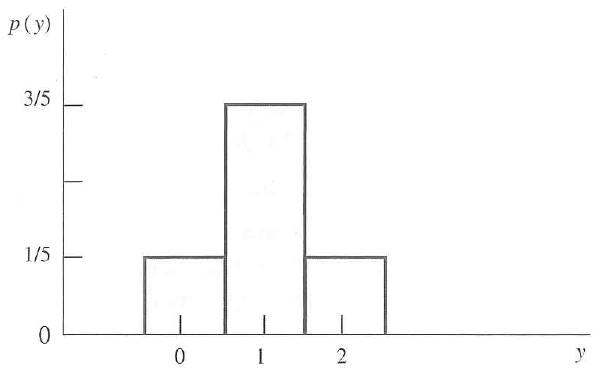
\includegraphics[width=0.3\textwidth]{pd1}
  \caption{A discrete probability distribution.\label{fig:pd1}}
\end{figure}

\begin{ex}\label{ex:pd1}
  A supervisor has three men and three women working for him. He chooses two of them at random for a particular job. Let $ W $ denote
  the number of women he chooses; we will find the probability distribution of $ W $.

  The supervisor can select two workers from six in $ \binom{6}{2} = 15 $ ways. Thus the sample space $ \Omega $ has 15 outcomes, each
  of which has probability $ 1/15 $ by assumption. The values for $ W $ which have non-zero probability are 0, 1, and 2; the number
  of ways of selecting $ W = 0 $ is $ \binom{3}{0} \binom{3}{2} = 3 $ (choose zero women from three and two men from three), and
  so $ p(0) = P(W = 0) = 3/15 $. Similarly, $ p(1) = \binom{3}{1}\binom{3}{1}/15 = 9/15 $, and $ p(2) = 3/15 $. Hence $ W = 1 $ is the most
  likely outcome, and the probability distribution is in \ref{fig:pd1}.
\end{ex}

The following facts are obvious:
\begin{prp}\label{prp:distfacts}\leavevmode
  \begin{enumerate}
    \item $ 0 \leq P(X = x) \leq 1 $ for any $ x $.
    \item If $ X $ can take the values $ x_1, ..., x_n, ... $ then $ P(X = x_1) + P(X = x_2) + \cdots + P(X = x_n) + \cdots = 1 $.
  \end{enumerate}
\end{prp}

\begin{defn}
  If $ X $ is a random variable on $ \Omega $ that takes numerical values, then the subset of elements $ \omega $ of $ \Omega $ such that $ x \leq X(\omega) \leq y $
  is called the event $ x \leq X \leq y $. The weak inequalities can be substituted with strong inequalities (${}<{}$) in the obvious fashion.
\end{defn}

The following theorem is obvious from the definition.
\begin{thm}[Discrete integration theorem]
  If a probability distribution is graphed, as in \ref{ex:pd1}, then $ P(x \leq X \leq y) $ is the area of the histogram
  bounded by $ x $ and $ y $ on the axis. More formally, $ P(x \leq X \leq y) = \rint_x^y X(\omega) \dif{\omega} $.
\end{thm}

\begin{exercise}\label{exercise:cointoss1}
  Alice and Bob play a game where each player tosses a fair coin. If the coins both come up
  tails, Alice wins \$1; if the coins both come up heads, Alice wins \$2; if the coins do not
  match, Alice loses \$1 (wins $-\$1$).

  Find the probability distribution for $ X $, Alice's expected winnings, after (a) a single
  play of the game; (b) five consecutive plays.
\end{exercise}

\subsection{Expected values}
\begin{defn}
  Let $ X $ be a discrete random variable, taking on the values $ x_1,...,x_n,...$, with probability function $ p(x) $. Then
  the \df{expected value} of $ X $ is defined to be $ E(X) = x_1 p(x_1) + \cdots + x_n p(x_n) + \cdots $.
\end{defn}

This `expectation' is a generalisation of the concept of \df{mean} that we have worked with since primary school. If
we consider the set $ \Omega = \{\omega_1,...,\omega_n\} $ then the mean of the set is
\begin{displaymath}
  \mu(\Omega) = \frac{1}{n} (\omega_1 + \cdots + \omega_n).
\end{displaymath}

Now suppose we define a function $ X $ from $ \Omega $ such that $ X(\omega_i) = \omega_i $ for each $ i $, and we
equip $ \Omega $ with the uniform probability function: that is, we set $ P(\omega_i) = 1/n $ for each $ i $.
I claim that $ E(X) = \mu(\Omega) $. Indeed,
\begin{displaymath}
  E(X) = \omega_1 P(\omega_1) + \cdots + \omega_n P(\omega_n) = \omega_1 (1/n) + \cdots + \omega_n (1/n) = \frac{1}{n} (\omega_1 + \cdots + \omega_n) = \mu(\Omega).
\end{displaymath}

Because of this, we will often write mean rather than expected value, and $ \mu(X) $ for $ E(X) $.

We are frequently interested in the average value (or more properly the expectation value) of some function of a random variable. For example,
molecules in space move at varying velocities; the velocity $ V $ is a random variable. Further, the kinetic energy $ E = \frac{1}{2} mV^2 $ is
a function of the random variable $ V $, and is therefore itself a random variable. Consequently, to find the mean amount of energy we need to
find the mean value of $ V^2 $.

\begin{thm}
  Let $ X $ be a real-valued discrete random variable, taking the values $ x_1,...,x_n $, with probability function $ p(x) $.
  Let $ g $ be a real-valued function that is defined on all the values of $ X $ (we will often abuse language and say that $ g $
  is a function defined on $ X $). Then the expected value of $ g(X) $ is
  \begin{displaymath}
    E[g(X)] = g(x_1) p(x_1) + \cdots + g(x_n) p(x_n)
  \end{displaymath}
\end{thm}
\begin{proof}[Proof (optional)]
  We will prove this in the case that $ X $ takes on only finitely many values, $ x_1,...,x_n $. Suppose $ g(X) $ takes on the distinct
  values $ g_1,...,g_m $, where $ m \leq n $ (since two different values of $ X $ might produce the same value of $ g(X) $). It
  follows that $ g(X) $ is a random variable satisfying $ P[g(y) = g_i] = \sum_{\substack{\text{all $ x_j $ such that}\\\text{$g(x_j) = g_i$}}} p(x_j) $ (where $ \Sigma $ is
  used to denote a sum);   denote the probability function of $ g(X) $ by $ p^* $. Then
  \begin{align*}
    E[g(X)] &= g_1 p^*(g_1) + \cdots + g_m p^*(g_m)\\
            &= g_1 \left(\sum_{\substack{\text{all $ x_j $ such that}\\\text{$g(x_j) = g_i$}}} p(x_j)\right) + \cdots + g_n \left(\sum_{\substack{\text{all $ x_j $ such that}\\\text{$g(x_j) = g_i$}}} p(x_j)\right)\\
            &= g(x_1) p(x_1) + \cdots + g(x_n) p(x_n).
  \end{align*}
\end{proof}

\begin{rem}
  The above theorem is actually true for \emph{every} discrete random variable; however, the proof becomes fiddly when the sums become
  infinite (one needs to check that they exist).
\end{rem}

Using our generalised mean, we will define a generalised standard deviation. Recall that the \df{variance} of
the set $ \Omega = \{\omega_1,...,\omega_n\} $ is the number
\begin{displaymath}
  \sigma^2(\Omega) = \frac{1}{n - 1}\left[(\omega_1 - \mu(\Omega))^2 + \cdots + (\omega_n - \mu(\Omega))^2\right]
\end{displaymath}
(that is, the sum of the squares of the differences between the measurements and their mean, divided by $ n - 1 $)
and the \df{standard deviation} of $ \Omega $ is just $ \sigma = \abs{\sqrt{\sigma^2(\Omega)}} $ (that is, the positive
square root of the deviance).

\begin{defn}
  If $ X $ is a standard variable with expectation $ E(X) = \mu $, the \df{variance} of $ X $ is defined to be
  the expected value of $ (X - \mu)^2 $. That is,
  \begin{displaymath}
    V(X) = E[(X - \mu)^2].
  \end{displaymath}
  The \df{standard deviation} of $ X $ is defined to be the positive square root of $ V(X) $.
\end{defn}

\begin{ex}
  A random variable $ X $ has the following probability distribution.
  \begin{center}
    \begin{tabular}{r|l}
      $ x $ & $ P(X = x) $\\\hline
      0 & $ 1/8 $ \\
      1 & $ 1/4 $ \\
      2 & $ 3/8 $ \\
      3 & $ 1/4 $
    \end{tabular}
  \end{center}

  Then
  \begin{displaymath}
    E(X) = 0(1/8) + 1(1/4) + 2(3/8) + 3(1/4) = 1.75,
  \end{displaymath}
  and
  \begin{multline*}
    V(X) = E((X - 1.75)^2)\\ = (0 - 1.75)^2 (1/8) + (1 - 1.75)^2 (1/4) + (2 - 1.75)^2 (3/8) + (3 - 1.75)^2 (1/4)\\ = 0.9375;
  \end{multline*}
  thus the mean is $ \mu = 1.75 $ and the standard deviation is $ \sigma = \sqrt{0.9375} = 0.968 $.

  Note that $ \mu \pm \sigma $ is the range $ 0.782 < X < 2.718 $, which includes 1 and 2 (i.e. over 62\% of the total probability
  distribution).
\end{ex}

We will now prove some simple rules for calculating combinations of expectation values.
\begin{prp}\label{prp:expectrules}
  Let $ X $ be a random variable, and let $ p(x) $ be the function $ P(X = x) $. Let $ g, g_1,...,g_n $ be functions of $ X $, and let $ \lambda $ be
  a constant. Then:
  \begin{enumerate}
    \item $ E(\lambda) = \lambda $
    \item $ E(\lambda g(X)) = \lambda E(g(X)) $
    \item $ E(g_1(X) + \cdots + g_n(X)) = E(g_1(X)) + \cdots + E(g_n(X)) $
  \end{enumerate}
  The final two statements together are called \df{linearity}.
\end{prp}
\begin{proof}
  Suppose $ X $ can take the values $ x_1,... $. Then:-
  \begin{enumerate}
    \item Note that $ \lambda $ is trivially a function of $ X $, and so $ E(\lambda) = \lambda P(x_1) + \cdots = \lambda(P(x_1) + \cdots) = \lambda $.
    \item $ E(\lambda g(X)) = \lambda g(x_1) P(x_1) + \cdots = \lambda(g(x_1) P(x_1) + \cdots) = \lambda E(g(X)) $.
    \item $ E(g_1(X) + \cdots + g_n(X)) = [g_1(x_1) + \cdots + g_n(x_1)] P(x_1) + \cdots = [g_1(x_1) P(x_1) + \cdots] + \cdots + [g_n(x_1) P(x_1)] = E(g_1(X)) + \cdots + E(g_n(X)) $.
  \end{enumerate}
\end{proof}

We may now give an easier method for calculating the variance of a discrete random variable.
\begin{prp}
  Let $ X $ be a random variable, and let $ p(x) $ be the function $ P(X = x) $. Let $ \mu = E(X) $,
  and let $ \sigma = +\sqrt{V(X)} $. Then:
  \begin{displaymath}
    V(X) = \sigma^2 = E[(X - \mu)^2] = E(X^2) - \mu^2.
  \end{displaymath}
\end{prp}
\begin{proof}
  The first two equalities are by definition, so we need to show that $ E[(X - \mu)^2] = E(X^2) - \mu^2 $. Applying
  the rules from proposition \ref{prp:expectrules} we find
  \begin{displaymath}
    E[(X - \mu)^2] = E(X^2 - 2\mu X + \mu^2) = E(X^2) + E(-2\mu X) + E(\mu^2) = E(X^2) - 2\mu E(X) + \mu^2
  \end{displaymath}
  and since $ E(X) = \mu $, $ E(X^2) - 2\mu E(X) + \mu^2 = E(X^2) - \mu^2 $.
\end{proof}

\begin{exercise}
  Recall from exercise \ref{exercise:cointoss1} that Alice and Bob were playing a game. Calculate
  the mean and variance of the random variable $ X $, Alice's winnings, after one play. How much
  should Alice pay to play a round of the game if her net winnings, the difference between the payoff
  and cost of playing, are to have mean 0?
\end{exercise}

\begin{exercise}
  Let $ X $ be a discrete random variable with mean $ E(X) = \mu $ and variance $ V(X) = \sigma^2 $. Define $ Y = X + 1 $.
  \begin{enumerate}
    \item Do you expect $ E(Y) $ to be larger than, equal to, or smaller than $ E(X) $? Why?
    \item Check your answer to 1. by writing $ E(Y + 1) $ in terms of $ E(X) $.
    \item Recalling that the variance is a measure of spread, do you expect $ V(Y) $ to be larger than, equal to, or smaller than $ V(X) $? Why?
    \item Use 2. to verify your expectation from 3.
  \end{enumerate}
\end{exercise}

\subsection{Binomial distributions}
The distribution we will consider now models a situation where a process is repeated, and each time only two outcomes
are possible. A production line produces a series of items, each either defective or nondefective; a
coin is flipped several times; a sequence of rocket launches either succeeds or fails.

\begin{defn}
  A \df{binomial distribution} is an experiment that consists of a fixed number $ n $ of identical trials, such that:
  \begin{enumerate}
    \item Each trial results in one of two outcomes, success or failure.
    \item The probability of success for each trial is equal to some value $ p $ that is constant across the experiment.
  \end{enumerate}
\end{defn}

\begin{thm}
  If an experiment satisfies the three conditions for a binomial distribution, with $ n $ trials and success probability $ p $,
  then the random variable $ X $ defined to be the number of successful trials, has the following probability function:
  \begin{displaymath}
    P(X = x) = \binom{n}{x} p^x (1-p)^{n-x}.
  \end{displaymath}
  This is called the probability function of the distribution.
\end{thm}
\begin{proof}
  Let $ \Omega $ be the sample space of the experiment; $ \Omega $ is the set of all strings of length $ n $ consisting
  of the characters $ S $ (success) and $ F $ failure. Then $ X(\omega) $ is the function that counts the number of instances
  of $ S $ in $ \omega $.

  We need to count the number of items in $ \Omega $ with $ x $ instances of $ S $. This is the same as picking, without
  replacement, $ x $ numbers from 1 to $ n $ (the numbers of the trials which succeed); i.e. there are $ \binom{n}{x} $
  such items. Further, the probability of each such item showing up is $ p^x (1 - p)^{n - x} $. The result follows.
\end{proof}

\begin{ex}
  If binary information is transmitted across an unreliable or noisy channel, we can model the probability
  that a single bit is incorrectly transmitted as a constant, $ p $. To improve reliability, we repeat each
  bit $ n $ times (where $ n $ is odd) and decide that the bit is 1 if a majority of the repeated digits arrive
  with value 1. If the probability $ p $ is constant over time, we have a binomial distribution with $ n $ trials
  and success probability $ p $ (where `success' means incorrect transmission).

  For a given message, we transmit each bit five times and there is a 10\% chance that any received bit has been
  changed in transmission (so $ n = 5 $ and $ p = 0.1 $). Then the probability a given bit is correctly received
  is the probability of at least three correct repeated bits; that is, the probability of at most two errors.

  This probability is just
  \begin{displaymath}
    P(X = 0) + P(X = 1) + P(X = 2) = \binom{5}{0} 0.1^0 0.9^{5-0} + \binom{5}{1} 0.1^1 0.9^{5-1} + \binom{5}{2} 0.1^2 0.9^{5-2} = 0.9914
  \end{displaymath}
  which is much better than $ p $.
\end{ex}

\begin{exercise}\leavevmode
  \begin{enumerate}
    \item Which is more likely: 9 heads in 10 tosses of a fair coin, or 18 heads in 20 tosses?
    \item Consider the binomial distribution of $ n $ trials and success probability $ p $, with probability function $ P(X = x) $. For what
          value $ k $ is $ P(X = k) $ maxmised? (Hint: consider $ P(X = k)/P(X = k+1) $.)
  \end{enumerate}
\end{exercise}

\section{Inference}
\textit{The primary reference for this section is Efron and Tibshirani.}
There are three basic questions to be asked in statistical investigations:
\begin{enumerate}
  \item How should I collect my data?
  \item How should I summarise the data I have collected?
  \item How accurate are my summaries?
\end{enumerate}
One tool to help answer the third question is the bootstrap, a comparatively modern methord for making
particular kinds of statistical inference. The calculations involved are intricate enough that they
are virtually impossible without a computer; the iNZight software can perform the relevant computations.\footnote{A
guide can be found at this URL: \url{https://www.stat.auckland.ac.nz/~wild/d2i/exercises/6.5\%20exercise-bootstrap-re-sampling_16.pdf}.}

A study\footnote{Efron and Tibshirani, pp.2--4} was performed in 1987 to see whether small aspirin doses
would prevent heart attacks in healthy middle-aged men. The data  were collecred by a controlled, randomised,
double-blind study. One half of the subjects reveived aspirin, the other half placebo; the subjects were
randomly assigned to the groups, and the supervising doctors were not told which group each subject was
assigned to. These precautions guard against seeing benefits that don't exist, while maximising the chance
of detecting a positive effect.

Here is a summary of the statistics that were measured:
\begin{center}
  \begin{tabular}{r|cc}
    & \textbf{heart attacks} & \textbf{subjects}\\\hline
    \textbf{aspirin} & 104 & 11037\\
    \textbf{placebo} & 189 & 11034
  \end{tabular}
\end{center}

We can calculate the relative risk that a person has a heart atach in the aspirin
group versus the placebo group fairly easily:
\begin{displaymath}
  \hat\rho = \frac{104/11037}{189/11034} - 0.55
\end{displaymath}
Thus if the study is reliable, the aspirin-takers have only 55\% as many heart attacks
as the placebo-takers.

In reality, we are not interested in the relative risk $ \hat\rho $ above --- it is only
the \emph{estimated} risk for this particular sample. Rather, we are interested in the relative
risk $ \rho $ for the entire population. Indeed, the sample here is large (over 22,000 subjects);
but the number of observed heart attacks is only 293.

It is possible to compute, using bootstraps, a confidence interval for the real value of $ \rho $:
we find that, with 95\% condidence, the real value lies within the interval
\begin{displaymath}
  0.43 < \rho < 0.70.
\end{displaymath}

The importance of confidence intervals is illustrated by another example from the same study. Here
is the data for strokes, measured for the same subjects as the heart attack table above.
\begin{center}
  \begin{tabular}{r|cc}
    & \textbf{heart attacks} & \textbf{subjects}\\\hline
    \textbf{aspirin} & 119 & 11037\\
    \textbf{placebo} & 98 & 11034
  \end{tabular}
\end{center}
Now the relative risk is estimated to be $ \hat\rho = 1.21 $: that is, taking aspirin seems be harmful! On the other
hand, if the confidence interval is calculated we find that $ 0.93 < \rho < 1.59 $. This range includes the neutral
value $ \rho = 1 $, and so it is impossible to say with any certainty whether aspiring is beneficial or harmful.

A bootstrap is a data-based simulation method for producing confidence intervals like these. The term comes from the
phrase `to pull oneself up by one's bootstraps'.\footnote{OED: To make use of existing resources or capabilities to raise (oneself)
to a new situation or state; to modify or improve by making use of what is already present.}

We will outline the process of boostrapping as it pertains to the stroke example. We create two populations: the first consisting of
119 ones and 11037 zeroes, and the second consisting of 98 ones and 11034 zeroes. We draw, with replacement, a sample of 11037 items
from the first population (sample A), and 11034 items from the second population (sample B). From these, we derive the \df{bootstrap replicant} of $ \hat \rho $:
\begin{displaymath}
  \hat \rho^* = \frac{\text{proportion of ones in sample A}}{\text{proportion of ones in sample B}}.
\end{displaymath}
We repeat this process a large number of times --- say 1000 times --- and end up with 1000 bootstrap replicants. These replicates contain
a large amount of information about the `shape' of the original data. For example, the standard deviation of the 1000 replicants generated
from the stroke data turned out to be 0.17; this is an estimate of the standard error of the relative risk $ \bar \rho $, and indicates that
the observed ratio of $ \hat \rho = 1.21 $ is only a little more than one standard error larger than 1; thus a value of $ \rho = 1 $ cannot
be ruled out.

To produce a rough 95\% confidence interval like $ 0.93 < \rho < 1.59 $, we simply take the 25th and 75th largest of the replicates (which
turned out to be 0.93 and 1.59).

(Why does this witchcraft work?!)

\section*{Bibliography and further reading}\phantomsection\addcontentsline{toc}{section}{Bibliography and further reading}
See references in text, as well as:
\begin{itemize}
  \item Bradley Efron and Robert J. Tibshirani, \textit{An introduction to the bootstrap}. Chapman \& Hall/CRC (1998).
  \item Mikl\'os B\'ona, \textit{A walk through combinatorics} (3e). World Scientific (2013).
  \item John A. Rice, \textit{Mathematical statistics and data analysis} (3e). Thomson Brooks/Cole (2007).
  \item Dennis D. Wackerly, William Mendenhall III, and Richard L. Sheaffer, \textit{Mathematical statistics with applications} (7e). Thomson Brooks/Cole (2008).
\end{itemize}

\end{document}
